\chapter{Background}
\label{ch:background}

\section{Chapter Overview}

In this chapter, we review some of the background critical to this report.

\section{Rhetorical Structure Theory (RST)}
The underlying principal of RST is that coherent texts consist of minimal units, which are linked to each other, recursively, through rhetorical relations \cite{Mann:1988}. Thus, the goal of RST is to describe the rhetorical organization of a text by using a hierarchical structure that captures the communicative intent of the writer. The first step in RST is to divide the text into elementary discourse units (EDUs), which generally correspond to clauses \footnote{Clauses that are subjects, objects,
or complements of a main verb are not treated as EDUs.}. Two adjacent EDUs are related to each other by a discourse relation. This relation is characterized as either paratactic or hypotactic. In the more common hypotactic relation, typically identified with subordination, the EDU that is more central to the text's purpose is labelled as the \textit{nucleus}, and the other (usually subordinating) EDU as the \textit{satellite}. In the paratactic relation, typically identified with coordination, all EDUs are labelled as \textit{nucleus}. These relations are then incrementally grouped together with other relations until forming a tree that spans the entire document.
Figure \ref{fig:background_rst} illustrates  examples of hypotactic relations on the left, and paratactic relations on the right.

\begin{figure}%
    \centering
    \subfloat[hypotactic]{{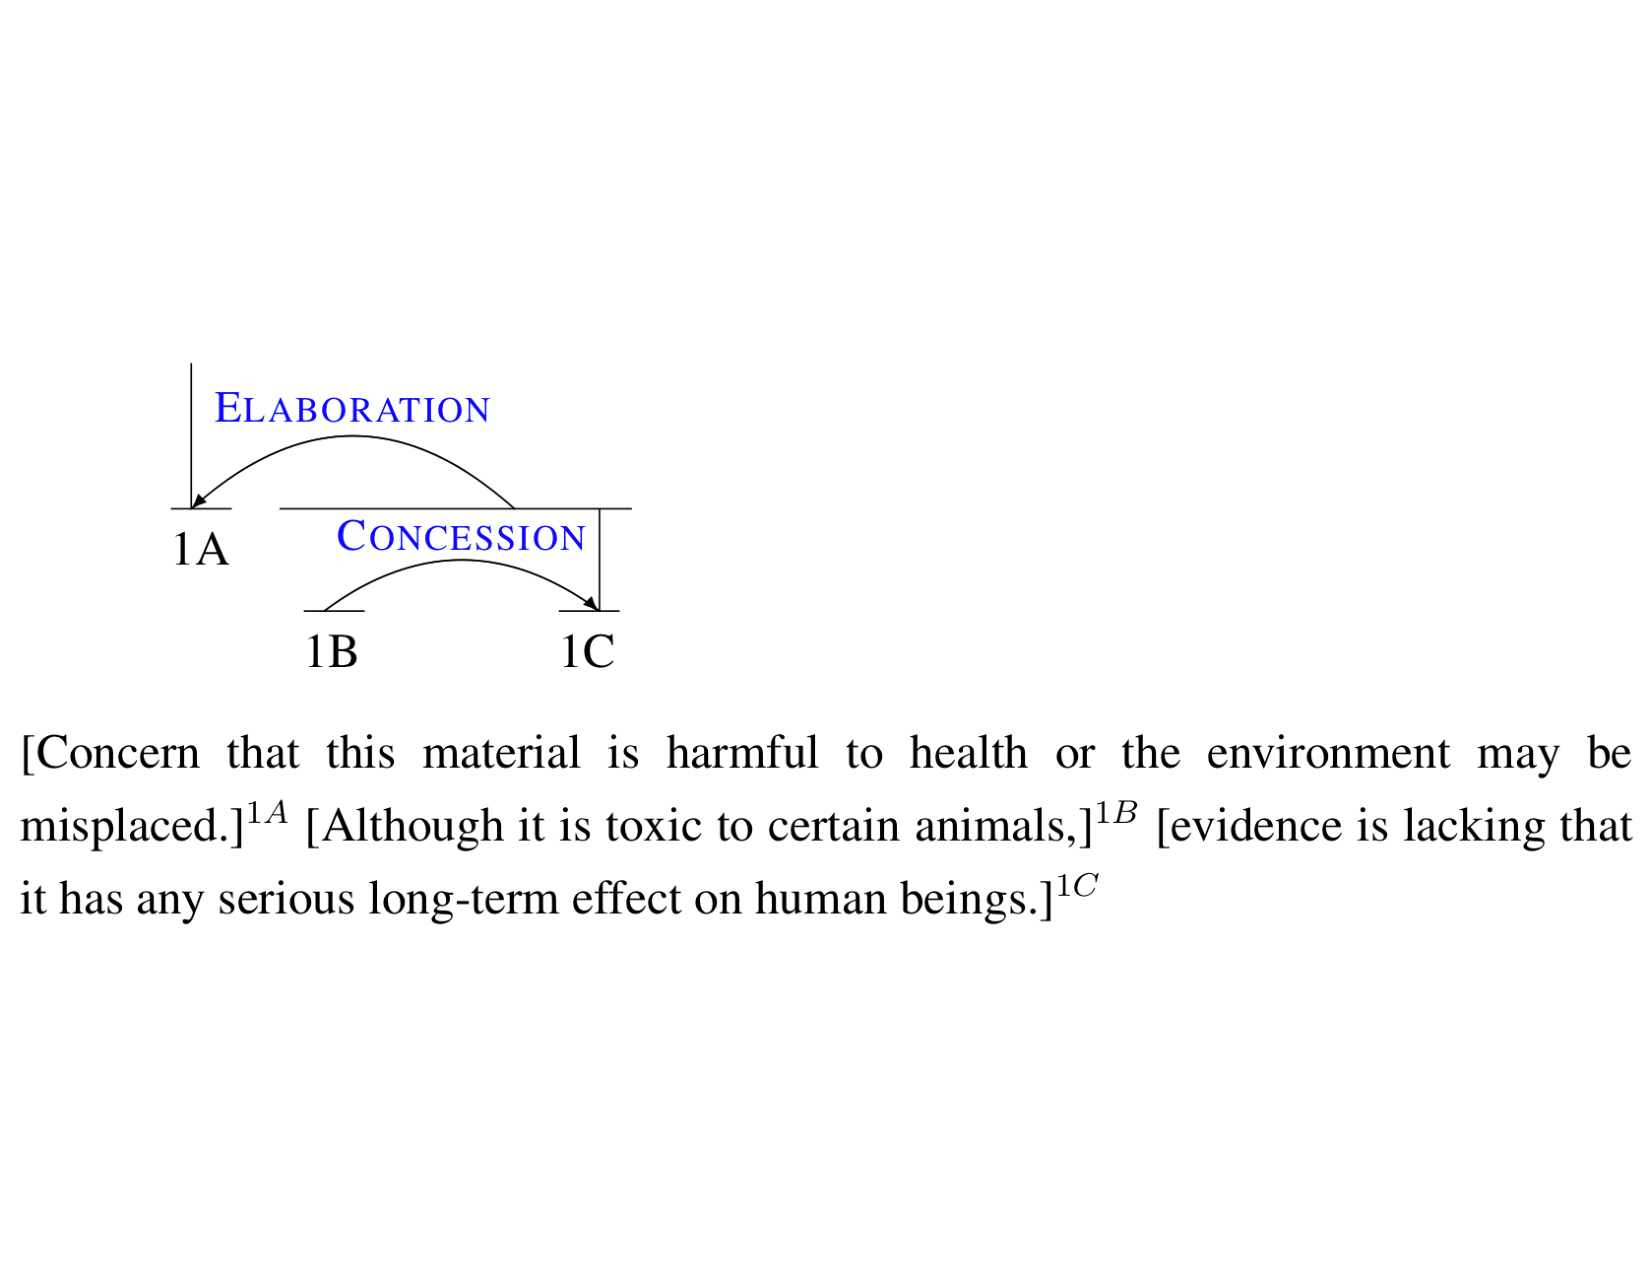
\includegraphics[width=10cm]{plots/rst-tree-1.pdf} }}%
    \qquad
    \subfloat[paratactic]{{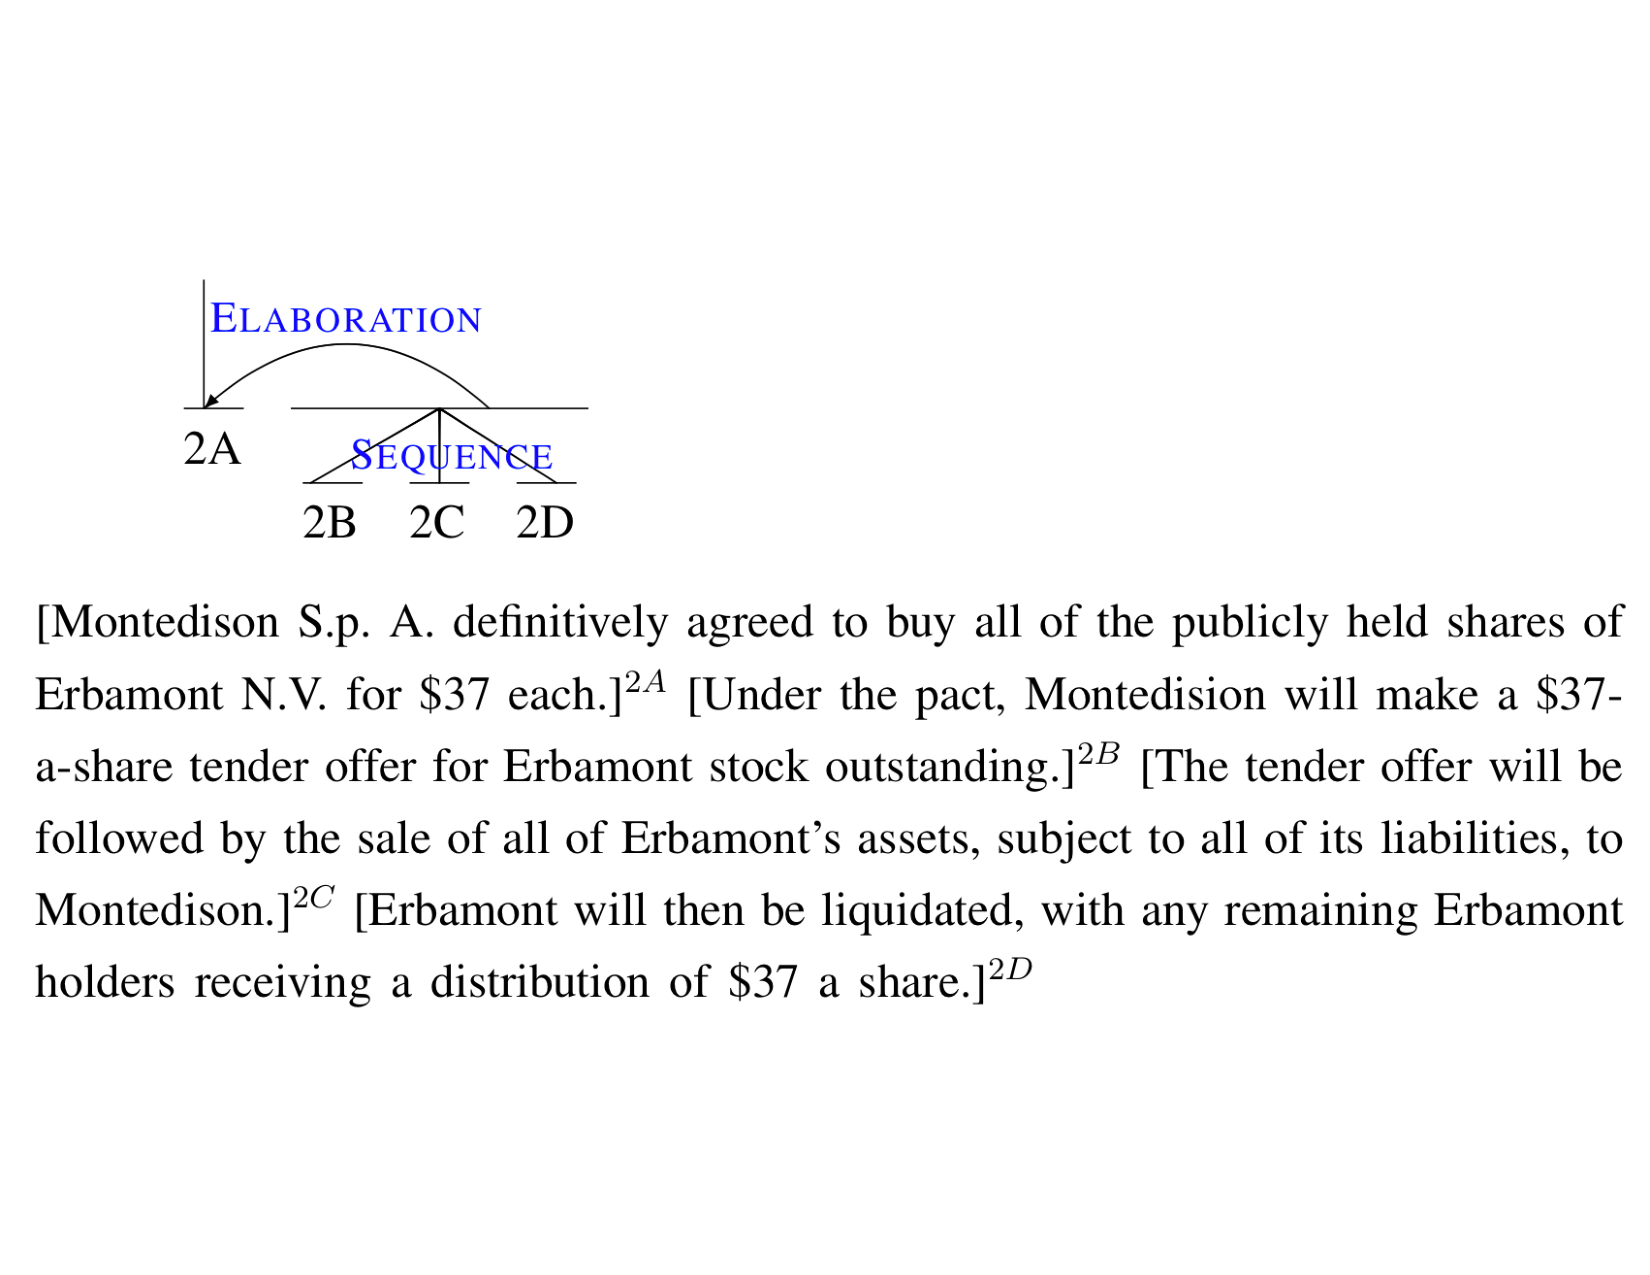
\includegraphics[width=10cm]{plots/rst-tree-2.pdf} }}%
    \caption{RST trees illustrating hypotactic and paratactic syntactic relations.}%
    \label{fig:background_rst}%
\end{figure}

%\dirrel{}
% {\rstsegment{\refr{txt1}}}{Elaboration}
% {
% \dirrel{Concession}{\rstsegment{\refr{txt2}}}
%    {}{\rstsegment{\refr{txt3}}}
% }
% \begin{rhetoricaltext}
%   \unit[txt1]{{Concern that this material is harmful to health %or the environment may be misplaced.}}
%   \unit[txt2]{{Although it is toxic to certain animals,}}
%   \unit[txt3]{{evidence is lacking that it has any serious long-term effect on human beings.}}
% \end{rhetoricaltext}
% \dirrel{}
% {
% \dirrel{}
% {
% \dirrel{}
% {
%  \dirrel{}
%  {
%   \dirrel{}
%   {\rstsegment{\refr{txt1}}}{Elaboration}
%   {\rstsegment{\refr{txt2}}}
%  }{Consequence}
%  {
%   \dirrel{}
%   {\rstsegment{\refr{txt3}}}{Elaboration}
%   {\rstsegment{\refr{txt4}}}
%  }
% }{Elaboration}
% {\rstsegment{\refr{txt5}}}
% }{Elaboration}
% {
%   \dirrel{}
%   {\rstsegment{\refr{txt6}}}{Elaboration}
%   {\rstsegment{\refr{txt7}}}
% }}{Elaboration}
% {
%   \dirrel{}
%   {\rstsegment{\refr{txt8}}}{Elaboration}
%   {\rstsegment{\refr{txt9}}}
% }

%  \begin{rhetoricaltext}
%   \unit[txt1]{{Emerson Electric Co. and Robert Bosch G.m.b. H. said the Federal Trade Commission has requested additional information from the two companies about their announced intention to acquire Vermont American Corp. for \$40 a share, or about \$440 million.}}
%   \unit[txt2]{{Yesterday, in composite trading on the American Stock Exchange, Vermont American common closed at \$39.75, off 25 cents.}}
%   \unit[txt3]{{The FTC's request was "not unusual" and Emerson will make a "full and prompt" response, according to a spokesman.}}
%   \unit[txt4]{{Spokesmen for Emerson and Vermont American, which has agreed to be acquired, said they don't anticipate "any problems" with the completion of the transaction.}}
%   \unit[txt5]{{An FTC spokesman said the matter is "in a non-public posture at this time" and declined to comment further.}}
%   \unit[txt6]{{Emerson and Bosch, through their joint acquisition arm, Maple Acquisition, have begun a cash tender offer for all of Vermont's common shares outstanding.}}
%   \unit[txt7]{{The offer, set to expire Nov. 1, may be extended pending the timing and resolution of the FTC request, the companies said.}}
%   \unit[txt8]{{St. Louis-based Emerson and Stuttgart-based Bosch make electrical and electronic products, including power tools.}}
%   \unit[txt9]{{The Vermont American acquisition is designed to enhance their position in the accessories portion of the power-tool industry.}}
%  \end{rhetoricaltext}

RST was operationalized in \newcite{Carlson:2001} with the RST Discourse Treebank (RST-DT).\footnote{\url{1https://catalog.ldc.upenn.edu/LDC2002T07}} This corpus consists of 385 Wall Street Journal articles from the Penn Treebank. Further research then proposed a set of rules to convert an RST tree into a dependency tree, where generally heads correspond to nuclear EDUs \cite{Hirao:2013}. 

With dependency trees being an appealing structure for computational models and the availability of the annotated corpus, RST has been widely adopted by the research community. In fact, RST has been shown to help with NLP tasks ranging from sentiment analysis to summarization, spanning domains such as online reviews and medical papers (\newcite{Ji:2017}, \newcite{Li:2016}, \newcite{Dacunha:2007}, \textit{interalia}). However, this same widespread use allowed the community to analyze its shortcomings, both in the theory and how it was operationalized. In our first study on discourse segmentation in the medical domain, we find evidence of problem areas for the way RST was operationalized.

\section{Structured Prediction and Attention}
\label{sec:structuredpred}
Statistical models can learn very well to detect patterns in large amounts of data. However, we also need to incorporate biases such as linguistic theories that help the model learn a task better. In this setting, the model predicts structured objects such as parse trees instead of scalars. 

With the shift to deep learning, research has focused more on models that learn latent representations of sentences or documents, constrained only by the end task. In our second study, we analyze one such model and attempt to incorporate some level of discourse theory. 

\section{Chapter Summary}

In this chapter, we described the two major concepts underpinning this report: RST and structured prediction. 


